\documentclass[10pt,twocolumn,letterpaper]{article}

\usepackage{cvpr}
\usepackage{times}
\usepackage{epsfig}
\usepackage{graphicx}
\usepackage{amsmath}
\usepackage{amssymb}

% Include other packages here, before hyperref.
%Path relative to the main .tex file 
\graphicspath{ {./images/} }

\usepackage{pgfplots}
\pgfplotsset{width=10cm,compat=1.9}

\usepgfplotslibrary{external}
\tikzexternalize

\usepackage{float} % https://tex.stackexchange.com/a/8633
\usepackage[skip=2pt]{caption} % https://tex.stackexchange.com/a/347975
\usepackage[skip=1ex, belowskip=2ex]{subcaption}
% If you comment hyperref and then uncomment it, you should delete
% egpaper.aux before re-running latex.  (Or just hit 'q' on the first latex
% run, let it finish, and you should be clear).
\usepackage[breaklinks=true,bookmarks=false]{hyperref}
\usepackage{tikz}
\usepackage[export]{adjustbox}

\cvprfinalcopy % *** Uncomment this line for the final submission

\def\cvprPaperID{****} % *** Enter the CVPR Paper ID here
\def\httilde{\mbox{\tt\raisebox{-.5ex}{\symbol{126}}}}

% Pages are numbered in submission mode, and unnumbered in camera-ready
%\ifcvprfinal\pagestyle{empty}\fi
\setcounter{page}{1}
\begin{document}

%%%%%%%%% TITLE
\title{Hair Product Recommendation System for Common Hair and Scalp Diseases}

\author{Joseph Yoo\\
Georgia State University\\
{\tt\small jyoo30@student.gsu.edu}
% For a paper whose authors are all at the same institution,
% omit the following lines up until the closing ``}''.
% Additional authors and addresses can be added with ``\and'',
% just like the second author.
% To save space, use either the email address or home page, not both
\and
Anirudha Narayanan\\
Georgia State University\\
{\tt\small anarayanan6@student.gsu.edu}
\and
Siya Katoch\\
Georgia State University\\
{\tt\small skatoch1@student.gsu.edu}
}


\maketitle
%\thispagestyle{empty}

%%%%%%%%% ABSTRACT
\begin{abstract}
Advancements in machine learning and computer vision have paved the way for sophisticated algorithms and models in medical diagnosis and treatment. This project focuses on leveraging convolutional neural networks (CNNs) to predict three common hair and scalp conditions from images and recommending appropriate treatments. These conditions include alopecia, psoriasis, and seborrheic dermatitis. Such work can assist those affected in early detection and treatment planning, as such conditions often progress without concern or ability to visit a professional for a diagnosis. The methodology includes data collection from diverse sources, preprocessing of the data, the testing of three popular pretrained convolutional image classification models, and a recommendation of treatment, given that a condition was predicted. The three models include ResNeXt, GoogLeNet, and AlexNet, and is used for our application, either through fine-tuning the models or using the models as a fixed-feature extractor. Augmentation using RandAugment was applied during training to expand the dataset and improve generalization of the models. Finally, a survey of treatments for the hair and scalp conditions was conducted and used to design a decision tree that could be used to recommend treatments given the prediction of a condition. Limited availability of accessible and uniform data made our task of classifying hair and scalp conditions difficult and made our task of learning treatments according to hair and scalp conditions infeasible. Across the three models and our tests, we achieved a maximum validation accuracy of 99\% and accuracies of 94.6\%, 100\%, 90.3\%, and 97.8\% for predicting alopecia, healthy, psoriasis, and seborrheic dermatitis, respectively, over all data.
\end{abstract}

%%%%%%%%% BODY TEXT
\section{Introduction}

Hair diseases can adversely impact an individual's quality of life, specifically their comfort and self-esteem. Identifying hair products relevant to specific hair diseases is crucial for providing appropriate treatment. This project proposes to leverage convolutional neural networks (CNNs) and modern deep learning techniques to determine a person's hair disease, or lack thereof, and recommend hair products to treat their condition appropriately.
%-------------------------------------------------------------------------
\section{Related Work}
Health evaluation is a long-time application of machine learning. Particularly, research into scalp damage recognition and hair disease identification using deep learning has begun relatively recently (2018, [5]). In a study by [1], physical and chemical analysis was conducted on 15,000 microscopic hair surface images to evaluate the degree of hair damage. A CNN, named SACN-Net, was then trained with 80\% of these evaluations to predict the degree of hair damage based on the hair surface images. SACN-Net utilizes residual connections, attention modules, and a global average pooling and performed better than several other CNN models, including ResNet50, with a test accuracy of 98.38\% on 20\% of the data.

Another study, by [2], used 70\% of a 150 scalp image dataset, collected from various sources, classified with alopecia, psoriasis, and folliculitis to train a CNN consisting solely of max pooling and convolution layers, with one fully connected (FC) layer before the output. Their model reached a “validation” (testing, in their case) accuracy of 91.1\% on 30\% of the data. 

A holistic, robust system, called ScalpEye, for efficient inspection and diagnosis of four common scalp hair symptoms, was developed by [3], which consists of a portable imaging microscope, mobile app, training server, and cloud management platform. They tested several popular models before settling on the R-CNN Inception ResNet\_v2\_Atrocious model for image recognition. ScalpEye was experimentally shown to diagnose dandruff, folliculitis, hair loss, and oily hair with an average precision of 97.41\% to 99.09\%.

Overall, an assortment of work has been conducted on the evaluation of scalp health and identification of scalp hair diseases, with many having impressive results. However, no studies on hair product recommendation systems were found. In this work, we will leverage and build upon the work of others and utilize these techniques to construct an effective hair treatment recommendation system.
%------------------------------------------------------------------------
\section{Data}
A drawback of deep learning is the large amount of data required for an accurate, but generalized model. Our dataset includes images labeled with hair and scalp conditions and healthy hair. Images labeled with hair and scalp conditions were collected from Kaggle, a data request, and a Github repository, originating from the DermNet and DermNetNZ dataset. Images labeled with healthy hair were collected from the Figaro 1K dataset.

\begin{figure}[H]
\centering
\begin{tabular}{ |c|c| }
\hline
 Label & Quantity \\
\hline
 Healthy & 1050 \\
 Alopecia & 147 \\
 Psoriasis & 134 \\
 Seborrheic Dermatitis & 90 \\
\hline
\end{tabular}
\captionof{table}{Images per Label}
\end{figure}
This data was preprocessed according to how the respective model was trained. This typically looks like a resizing, central crop, and normalization using a mean and standard deviation of ImageNet [8]. During training, an augmentation technique called RandAugment [9] was applied to the batches.
%------------------------------------------------------------------------
\section{Methodology}
\subsection{Model}
As aforementioned, data will be preprocessed according to conventional techniques for transfer learning. This process is shown in Fig. 1. The standard ImageNet transforms include a resizing to 256x256 pixels using billinear interpolation, a central crop to 224x224 pixels, and a normalization to the mean and standard deviation of the dataset. During training, augmentation is applied to batches of images using RandAugment. This technique chooses and applies some number of randomly chosen transformations at some severity. The number of transformations and their severity are two hyper-parameters of a hyper-parameter search problem based on validation accuracy [9].
\begin{figure}[htp]
  % Equal length
  \hspace*{\fill}%
  \subcaptionbox{Original\label{fig1:a}}{\includegraphics[scale=0.15]{sample_image}}\hfill%
  \subcaptionbox{Transformed\label{fig1:b}}{\includegraphics[scale=0.3]{transformed_image}}%
  \hfill%
  \subcaptionbox{Transformed and Augmented\label{fig1:c}}{\includegraphics[scale=0.3]{latex/images/transformed_augmented_image.jpg}}%
  \hspace*{\fill}%
\caption{Image Preprocessing}
\end{figure}

One of the factors that the generalization of a deep learning model depends on is the balanced-ness of the dataset. A great imbalance risks the model developing a bias for the majority label(s). If so, a model may exhibit a high accuracy, but a confusion matrix will reveal that the model performs well only on the biased labels. Given that a majority of our data is labeled as "Healthy", our model is likely to develop a bias for that label. A variety of techniques exist to circumvent this issue. We will compare three techniques: a control, sampling with respect to the inverse frequency of the labels, and a modified loss function. In the control, batches will be sampled with an assumption that the data is balanced. Sampling with respect to the inverse frequency of the labels is based on the technique of under-and-oversampling, pulling more images from the under-represented labels and less images from the over-represented labels, relative to the control. The modified loss function is a multi-class implementation of a technique called focal loss [13]. Simply put, it can be thought to "encourage" the model to prefer the predictions of false positives over false negatives (i.e. predicting a condition when there is none is preferable to predicting no condition when there is one).

We will apply transfer learning to three different popular pre-trained models to classify hair and scalp conditions. These models include ResNeXt [7], GoogLeNet [10], and AlexNet [12], and all utilize convolutions. ResNeXt builds upon... The best performing weights of each model will be saved and compared. The best performing model will be used for the condition classifier of the hair and scalp treatment recommendation system.

For transfer learning, we can either fine-tune the model and using the model as a fixed-feature extractor. Considering that the new dataset is small and different from the original dataset (ImageNet), we should use the model as a fixed-feature extractor to avoid over-fitting [11]. However, we will try both techniques and compare their performances.

\subsection{Treatment Recommendation}

%------------------------------------------------------------------------
\section{Experiments and Results}

\begin{figure}[H]
\centering
\begin{tabular}{ |c|c|c| }
\hline
 ResNext-50 & 96\% \\
\hline
 GoogLeNet & 99\% \\
\hline
 AlexNet & 90\% \\
\hline
\end{tabular}
\captionof{table}{Model \& Validation Accuracy}
\end{figure}

\begin{figure}[H]
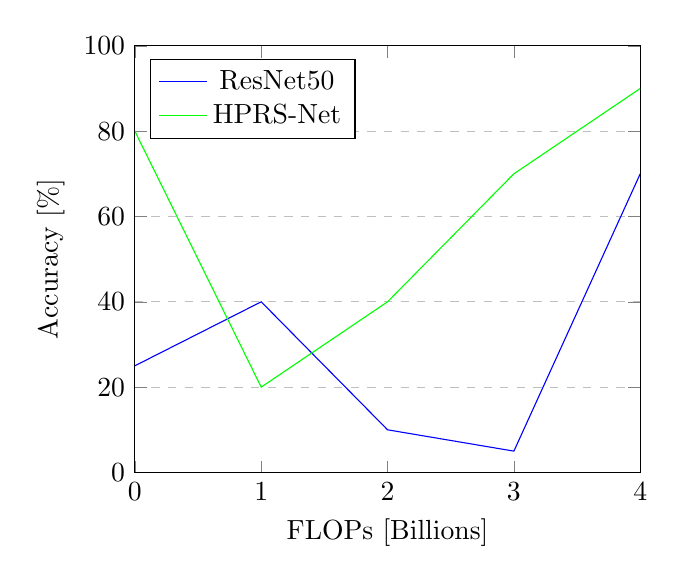
\begin{tikzpicture}
\begin{axis}[
    % title={Accuracy of Models to FLOPs},
    width=8cm,height=7cm,
    xlabel={FLOPs [Billions]},
    ylabel={Accuracy [\%]},
    xmin=0, xmax=4,
    ymin=0, ymax=100,
    xtick={0,1,2,3,4},
    ytick={0,20,40,60,80,100},
    legend pos=north west,
    ymajorgrids=true,
    grid style=dashed,
]

\addplot[
    color=blue,
    ]
    coordinates {
    (0,25)(1,40)(2,10)(3,5)(4,70)
    };
\addplot[
    color=green,
    ]
    coordinates {
    (0,80)(1,20)(2,40)(3,70)(4,90)
    };
\legend{ResNet50, HPRS-Net}
\end{axis}
\end{tikzpicture}
\caption{Model FLOPs to Accuracy}
\end{figure}

As seen in Table 1, HPRS-Net outperforms ResNet50, a general purpose image classifier, and SACN-Net, a scalp image classifier. Furthermore, our model is more efficient than ResNet50, as seen in Figure 1.
%------------------------------------------------------------------------
\section{Conclusions}
We do not have any results to conclude from.
%------------------------------------------------------------------------
{\small
\nocite{*}
\bibliographystyle{ieee_fullname}
\bibliography{CS4851}
}

\end{document}
